\subsection{Basic Geometric Concepts}
\label{math-obj}

This chapter introduces the main geometric concepts considered necessary to
provide a solid understanding of SS-LLE\footnote{
Obviously, the list of concepts discussed is by no means extensive. Theory is
presented much more in detail (and mathematical rigor) in, for example, 
\textcolor{red}{good book}.
}.
It must be noted that everything discussed here is presented through the lens of
machine learning, deliberately forsaking the generality inherent to topology.
Therefore, assuming features can be represented by coordinates in 
$D$-dimensional Euclidean space, all concepts are examined with regard to their
meaning in $\RD$.
Dimensionality reduction techniques take the data observed in $\RD$ to actually
lie in a $d$-dimensional topological space that is not necessarily Euclidean but
exhibits some specific properties.
\\

% FIXME Make enumeration more compact 

\textbf{Topological spaces.} A \textit{topological space} is constituted by a 
set $X$ equipped with a \textit{topology} $\topo$. 
A topology is a general way of describing relations between elements in $X$.
Consider a function $\topo: X \rightarrow 2^X, x \mapsto \topo(x)$, which 
assigns to $x \in X$ a set of subsets of $X$ called a \textit{neighborhood}.
For $\topo$ to be a topology\footnote{
Alternative definitions employ open subsets of $X$, see for example 
\citet{waldmann2014}.
}
on $X$, the following properties must hold \citep{brown2006}:
\begin{tight_enumerate}
  \item If $\topo$ is a neighborhood of $x$, then $x \in \topo$.
  \item If $\topo$ is a subset of $X$ containing a neighborhood of $x$, then 
  $\topo$ is a neighborhood of $x$.
  \item The intersection of two neighborhoods of $x$ is again a neighborhood to
  $x$.
  \item Any neighborhood $\topo$ of $x$ contains a neighborhood $\topo^{\prime}$ 
  of $x$ such that $\topo$ is a neighborhood of each element in 
  $\topo^{\prime}$.
\end{tight_enumerate}

Note that, in this general definition, neighborhoods are based on an abstract
notion of "nearness". 
Learning the structure of a topological space effectively boils down to learning 
neighborhood relations.
In Euclidean topological space these are directly based on distance: 
neighborhoods are constructed by $\epsilon$-balls containing all elements within 
a Euclidean distance of $\epsilon$ from $x$. 
The resulting topology is also called the \textit{metric topology} 
\citep{mccleary2006}.

Topological spaces in general are not accessible via distances.
The ultimate goal is again the interpretation of the data in a Euclidean space, 
albeit one with lower dimensionality, where such concepts are meaningful.
The next step is thus to study how a (potentially highly non-linear and
complicated) topological space might relate to $\Rd$.
\\

\textbf{Homeomorphisms.} Consider two topological spaces $(X, \topo_X)$, 
$(Y, \topo_Y)$ (denoted by the respective shorthands $X$, $Y$ from here) and a 
mapping function $f: X \rightarrow Y$. 
If $f$ is bijective and continuous and $f^{-^1}: Y \rightarrow X$ is also 
continuous, $f$ is called a \textit{homeomorphism}.
Intuitively, this is equivalent to $f(\topo)$ being a neighborhood of $f(x)$ if
$\topo$ is a neighborhood of $x$ \citep{brown2006}.
Topological spaces for which such a mapping exists are \textit{homeomorphic} to
each other. 
Any properties of $X$ that $Y$ shares when it is homeomorphic to $X$ are 
referred to as topological properties. 
Two homeomorphic spaces are thus topologically equivalent \citep{mccleary2006}.

If there exists a non-negative integer $d$ such that for every $x$ in a 
topological space $X$ a local neighborhood is homeomorphic to an open subset of 
$\Rd$, $X$ is \textit{locally Euclidean}\footnote{
For locally Euclidean topological spaces it is thus meaningful to speak of
elements as points.
}.
In local neighborhoods $X$ then behaves like $\Rd$, which is conceivably a 
desirable property in this context \citep{mafu2011}.
\\

\textbf{Manifolds.} \textit{Manifolds} are now precisely such locally Euclidean
topological spaces, with some additional properties.
For $\mani$\footnote{
This is again a shorthand, omitting the explicit notation of the corresponding
topology to enhance readability. 
} to be a $d$-dimensional manifold (also: $d$-manifold) it must meet 
the following conditions \citep{waldmann2014}:

\begin{tight_enumerate}
  \item $\mani$ is Hausdorff.
  \item $\mani$ is second-countable.
  \item $\mani$ is locally homeomorphic to $\Rd$.
\end{tight_enumerate}

The Hausdorff condition is a separation property and ensures that for any two 
distinct points from $\mani$ disjoint neighborhoods can be found 
\citep{brown2006}.
Second-countability restricts the manifold's size via the number of open sets 
it may possess \citep{waldmann2014}.

Manifolds can now be \textit{embedded} in Euclidean space.
Consider $\R^k \supset \Rd$\footnote{
Here, $k$ is used to denote a general higher-dimensional space (a manifold
embedded in $\R^k$ is also embedded in $\R^{k + 1}$, and so on, as 
homeomorphisms are transitive \citep{waldmann2014}). 
This is deliberate to distinguish it from the more specific notation $D$ 
indicating the number of observed features.
}.
$\Rd$ is endowed with the so-called \textit{subspace topology} that results
from intersecting open subsets of $\R^k$ with $\Rd$ (for $\R^2$, these are
$\epsilon$-circles obtained by intersecting $\R^3$-$\epsilon$-balls with the 
coordinate planes).
For a manifold $\mani$ to be embedded in $\R^k$ means that $\mani$ is enclosed
by $\R^k$ but locally homeomorphic to $\Rd$, thereby inheriting the metric
subspace topology from $\Rd$ \citep{waldmann2014}.
It can be shown that $k = 2d + 1$ is sufficient to create an embedding, but $k$
may be smaller \citep{mafu2011}.

This now has important consequences for manifold learning: data lying on a 
$d$-dimensional manifold $\mani$ embedded in $\mathbb{R}^k$ are observed as 
$k$-dimensional points but may locally be treated like points from $\Rd$.
\\

Figure \ref{fig:scurve} shows the well-known \textit{S-curve} manifold embedded 
in $\R^3$.
Clearly, the S-curve as a whole is far from linear, but local patches on its
surface behave like flat surfaces from $\R^2$.
So the S-curve is two-dimensional and feature dimensionality can in effect be 
compressed from $\R^3$ to $\R^2$.
The challenge is now to unravel the manifold in a way that preserves its 
structure to maximum extent.
Obviously, a simple projection to $\R^2$ (onto any coordinate plane) will not
accomplish this task.
Instead, manifold learning must capture the intrinsic neighborhood structures
and map these to $\R^2$, which, in this case, can be imagined as a 
"flattening-out" of the S-curve.

\begin{figure}[H]
  \centering
  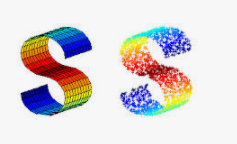
\includegraphics[width = 0.8\textwidth]{figures/s-curve-screenshot}
  \caption[S-curve manifold]{XY points sampled from the S-curve manifold,
  obtained by bla.}
  \label{fig:scurve}
\end{figure}

\textbf{Geodesic.} One last aspect remains open, namely how to handle distances 
on manifolds.
Figure \ref{fig:scurve} illustrates that standard Euclidean distances are not
meaningful here: rather than measuring "shortcuts" between points across 
$\R^3$ (where, for instance, points in the upper blue area would be considered
quite close to points in the red area), it makes intuitive sense to constrain 
distances to the manifold surface.
In order to enable the construction of such a metric, manifolds must fulfill
two additional properties: being \textit{Riemannian} and being 
\textit{connected} \citep{mafu2011}.

\textcolor{red}{Riemannian manifolds are differentiable}

Connectedness means that no separation $\{ U, V\}$ of a manifold $\mani$
exists with open, non-empty and disjoint $U, V \subset \mani$, 
$\mani = U \cup V$.
For manifolds, connectedness is immediately equivalent with path-connectedness,
which is perhaps more intuitive: informally stated, any two points on a 
connected manifold can be linked by a path
% Such a path is a continuous function $\lambda: [0, 1] \rightarrow \mani$ with
% $\lambda(x) = 0$ and $\lambda(y) = 1$ for any two points $x, y \in \mani$
\citep{mccleary2006}.

For connected Riemannian manifolds it is now possible to define a distance 
metric, or \textit{geodesic distance}.
Geodesic distance is the length of the shortest curve (\textit{geodesic}) on
$\mani$ between two points $\pv, \qv \in \mani$, as measured by arc-length (such 
a curve must exist due to connectedness)\footnote{
Geodesics are but a peripheral note here; for a precise definition see for 
example \citet{mafu2011}.
}.


% A curve $c$ in $\mani$ is a smooth mapping from an open interval 
% $\Lambda \subset \R$ into $\mani$. 
% $c$ is parametrized by a point $\lambda \in \Lambda$, such that 
% $c(\lambda) = (c_1(\lambda), ..., c_d(\lambda))^T$ (all $c_j, j = 1, ..., d$,
% having a sufficient number of continuous derivatives) is a curve in $\Rd$.
% Component-wise differentiation with respect to $\lambda$ yields the 
% \textit{velocity} of $c$ in $\lambda$, $c^{\prime}(\lambda) =
% (c_1^{\prime}(\lambda), ..., c_d^{\prime}(\lambda))^T$.
% The \textit{speed} of $c$ is given by $\| c^{\prime}(\lambda) \|^2_2$, where
% $\| \cdot \|^2_2$ denotes the square norm.
% Then, distance along this curve is measured by the arc-length 
% $L(c) = \int_{\pv}^{\qv} \| c^{\prime}(\lambda) \|^2_2 d\lambda$.
% 
% Finally, geodesic distance can be derived as the length of the shortest such
% curve, out of the set of differentiable curves in $\mani$ that connect $\pv$ and 
% $\qv$, $\mathcal{C}(\pv, \qv)$: \\
% $d^{\mani}(\pv, \qv) = \inf_{c \in \mathcal{C}(\pv, \qv)} L(c)$ 
% \citep{mafu2011}. 

Intuitively, geodesic distance can be identified with Euclidean distance in
Euclidean spaces where shortest curves are but straight lines \citep{mafu2011}.

\subsection{Spectral Decomposition}
\label{spect-dec}

\begin{itemize}
  \item Eigenvalues/eigenvectors 
  \item Spectral decomposition
\end{itemize}


